
%%% main document {{{

\documentclass[
a4paper,     %% defines the paper size: a4paper (default), a5paper, letterpaper, ...
% landscape,   %% sets the orientation to landscape
% twoside,     %% changes to a two-page-layout (alternatively: oneside)
% twocolumn,   %% changes to a two-column-layout
 headsepline, %% add a horizontal line below the column title
% footsepline, %% add a horizontal line above the page footer
% titlepage,   %% only the titlepage (using titlepage-environment) appears on the first page (alternatively: notitlepage)
% parskip,     %% insert an empty line between two paragraphs (alternatively: halfparskip, ...)
% leqno,       %% equation numbers left (instead of right)
% fleqn,       %% equation left-justified (instead of centered)
% tablecaptionabove, %% captions of tables are above the tables (alternatively: tablecaptionbelow)
% draft,       %% produce only a draft version (mark lines that need manual edition and don't show graphics)
% 10pt         %% set default font size to 10 point
11pt         %% set default font size to 11 point
% 12pt         %% set default font size to 12 point
]{scrartcl}  %% article, see KOMA documentation (scrguide.dvi)



%%%%%%%%%%%%%%%%%%%%%%%%%%%%%%%%%%%%%%%%%%%%%%%%%%%%%%%%%%%%%%%%%%%%%%%%%%%%%%%%
%%%
%%% packages
%%%

%%%
%%% encoding and language set
%%%

%%% ngerman: language set to new-german
\usepackage{ngerman}

%%% babel: language set (can cause some conflicts with package ngerman)
%%%        use it only for multi-language documents or non-german ones
%\usepackage[ngerman]{babel}

%%% inputenc: coding of german special characters
\usepackage[utf8]{inputenc}

%%% fontenc, ae, aecompl: coding of characters in PDF documents
\usepackage[T1]{fontenc}
\usepackage{ae,aecompl}

%%%
%%% technical packages
%%%

%%% amsmath, amssymb, amstext: support for mathematics
%\usepackage{amsmath,amssymb,amstext}

%%% psfrag: replace PostScript fonts
\usepackage{psfrag}

%%% listings: include programming code
%\usepackage{listings}

%%% units: technical units
\usepackage{units}

%%% tiefgestellte zahlen
\usepackage{subscript}

%%% mathefoo
\usepackage{amsmath}

%%% landscape page
\usepackage{pdflscape}

%%% multirow table stuff
\usepackage{multirow}
\usepackage{array}

\usepackage{xcolor}
% TikZ-Bibliotheken
\usepackage{tikz}
 \usetikzlibrary{backgrounds}
 \usetikzlibrary{matrix}
 \usetikzlibrary{circuits.ee.IEC}
 \usetikzlibrary{circuits.logic.IEC}
 \usetikzlibrary{positioning}
 
 
%Hintergrundstyle - optional
\tikzstyle{background rectangle}=
  [thick,draw=\lightgray, fill=white!99!black, rounded corners]
 
%Volt- und Amperemeter festlegen:
\tikzset{circuit declare symbol = ammeter}
\tikzset{set ammeter graphic ={draw,generic circle IEC, minimum size=5mm,info=center:A}}
\tikzset{circuit declare symbol = voltmeter}
\tikzset{set voltmeter graphic ={draw,generic circle IEC, minimum size=5mm,info=center:V}}
\tikzset{circuit declare symbol = generator}
\tikzset{set generator graphic ={draw,rectangle ee, minimum size=5mm,info=center:G}}

%%%%%%%%%%%%%%%%%%%%%%%%%%%%%%%%%%%%%%%%%%%%%%%%%%%%%%%%%%%%%%%%%%%%%%%%%%
% Transistor Platzhalter, bitte durch echten Transistor ersetzen
\tikzset{circuit declare symbol = transistor}
\tikzset{set transistor graphic ={draw,generic circle IEC, minimum size=5mm,info=center:T}}
%%%%%%%%%%%%%%%%%%%%%%%%%%%%%%%%%%%%%%%%%%%%%%%%%%%%%%%%%%%%%%%%%%%%%%%%


% Spannungs und Strompfeile
\tikzset{
  Pfeil/.style={thick,shorten >=#1,shorten <=#1,->}, % für Peile
  UPfeil/.style={blue,Pfeil=#1,font={\sffamily\itshape}},% für Spannungspfeile
  IPfeil/.style={red,Pfeil=#1,font={\ttfamily\itshape}} % für Strompfeile
}


%\usepackage{circuitikz}

%Boxen
\usepackage{empheq}
 
% Command "alignedbox{}{}" for a box within an align environment
% Source: http://www.latex-community.org/forum/viewtopic.php?f=46&t=8144
\newlength\dlf  % Define a new measure, dlf
\newcommand\alignedbox[2]{
% Argument #1 = before & if there were no box (lhs)
% Argument #2 = after & if there were no box (rhs)
&  % Alignment sign of the line
{
\settowidth\dlf{$\displaystyle #1$}  
    % The width of \dlf is the width of the lhs, with a displaystyle font
\addtolength\dlf{\fboxsep+\fboxrule}  
    % Add to it the distance to the box, and the width of the line of the box
\hspace{-\dlf}  
    % Move everything dlf units to the left, so that & #1 #2 is aligned under #1 & #2
\boxed{#1 #2}
    % Put a box around lhs and rhs
}
}

%%%
%%% layout
%%%

%%% scrpage2: KOMA heading and footer
%%% Note: if you don't use this package, please remove 
%%%       \pagestyle{scrheadings} and corresponding settings
%%%       below too.
\usepackage[automark]{scrpage2}


%%%
%%% PDF
%%%

\usepackage{ifpdf}

%%% Should be LAST usepackage-call!
%%% For docu on that, see reference on package ``hyperref''
\ifpdf%   (definitions for using pdflatex instead of latex)

  %%% graphicx: support for graphics
  %\usepackage[pdftex]{graphicx}

  \pdfcompresslevel=9

  %%% hyperref (hyperlinks in PDF): for more options or more detailed
  %%%          explanations, see the documentation of the hyperref-package
  \usepackage[%
    %%% general options
    pdftex=true,      %% sets up hyperref for use with the pdftex program
    %plainpages=false, %% set it to false, if pdflatex complains: ``destination with same identifier already exists''
    %
    %%% extension options
    backref,      %% adds a backlink text to the end of each item in the bibliography
    pagebackref=false, %% if true, creates backward references as a list of page numbers in the bibliography
    colorlinks=true,   %% turn on colored links (true is better for on-screen reading, false is better for printout versions)
    %
    %%% PDF-specific display options
    bookmarks=true,          %% if true, generate PDF bookmarks (requires two passes of pdflatex)
    bookmarksopen=false,     %% if true, show all PDF bookmarks expanded
    bookmarksnumbered=false, %% if true, add the section numbers to the bookmarks
    %pdfstartpage={1},        %% determines, on which page the PDF file is opened
    pdfpagemode=None         %% None, UseOutlines (=show bookmarks), UseThumbs (show thumbnails), FullScreen
  ]{hyperref}


  %%% provide all graphics (also) in this format, so you don't have
  %%% to add the file extensions to the \includegraphics-command
  %%% and/or you don't have to distinguish between generating
  %%% dvi/ps (through latex) and pdf (through pdflatex)
  \DeclareGraphicsExtensions{.pdf}

\else %else   (definitions for using latex instead of pdflatex)

  \usepackage[dvips]{graphicx}

  \DeclareGraphicsExtensions{.eps}

  \usepackage[%
    dvips,           %% sets up hyperref for use with the dvips driver
    colorlinks=false %% better for printout version; almost every hyperref-extension is eliminated by using dvips
  ]{hyperref}

\fi


%%% sets the PDF-Information options
%%% (see fields in Acrobat Reader: ``File -> Document properties -> Summary'')
%%% Note: this method is better than as options of the hyperref-package (options are expanded correctly)
\hypersetup{
  pdftitle={}, %%
  pdfauthor={}, %%
  pdfsubject={}, %%
  pdfcreator={Accomplished with LaTeX2e and pdfLaTeX with hyperref-package.}, %% 
  pdfproducer={}, %%
  pdfkeywords={} %%
}


%%%%%%%%%%%%%%%%%%%%%%%%%%%%%%%%%%%%%%%%%%%%%%%%%%%%%%%%%%%%%%%%%%%%%%%%%%%%%%%%
%%%
%%% user defined commands
%%%

%%% \mygraphics{}{}{}
%% usage:   \mygraphics{width}{filename_without_extension}{caption}
%% example: \mygraphics{0.7\textwidth}{rolling_grandma}{This is my grandmother on inlinescates}
%% requires: package graphicx
%% provides: including centered pictures/graphics with a boldfaced caption below
%% 
\newcommand{\mygraphics}[3]{
  \begin{center}
    \includegraphics[width=#1, keepaspectratio=true]{#2} \\
    \textbf{#3}
  \end{center}
}

%%%%%%%%%%%%%%%%%%%%%%%%%%%%%%%%%%%%%%%%%%%%%%%%%%%%%%%%%%%%%%%%%%%%%%%%%%%%%%%%
%%%
%%% define the titlepage
%%%

% \subject{}   %% subject which appears above titlehead
% \titlehead{} %% special heading for the titlepage

%%% title
\title{Messbericht \\ Digitaltechnik Teil 1}

%%% author(s)
\author{Felix Schiller \\ Sebastian Littau \\ E1FS2}

%%% date
\date{Reutlingen, am 10.05.2016}

% \publishers{}

% \thanks{} %% use it instead of footnotes (only on titlepage)

% \dedication{} %% generates a dedication-page after titlepage


%%% uncomment following lines, if you want to:
%%% reuse the maketitle-entries for hyperref-setup
%\newcommand\org@maketitle{}
%\let\org@maketitle\maketitle
%\def\maketitle{%
%  \hypersetup{
%    pdftitle={\@title},
%    pdfauthor={\@author}
%    pdfsubject={\@subject}
%  }%
%  \org@maketitle
%}


%%%%%%%%%%%%%%%%%%%%%%%%%%%%%%%%%%%%%%%%%%%%%%%%%%%%%%%%%%%%%%%%%%%%%%%%%%%%%%%%
%%%
%%% set heading and footer
%%%

%%% scrheadings default: 
%%%      footer - middle: page number
\pagestyle{scrheadings}

%%% user specific
%%% usage:
%%% \position[heading/footer for the titlepage]{heading/footer for the rest of the document}

%%% heading - left
\ihead[]{Schiller, Felix \\ Littau, Sebastian}

%%% heading - center
\chead[]{Messbericht \\ Digitaltechnik Teil 1}

%%% heading - right
\ohead[]{\thepage}

%%% footer - left
% \ifoot[]{}

%%% footer - center
% \cfoot[]{}

%%% footer - right
% \ofoot[]{}



%%%%%%%%%%%%%%%%%%%%%%%%%%%%%%%%%%%%%%%%%%%%%%%%%%%%%%%%%%%%%%%%%%%%%%%%%%%%%%%%
%%%
%%% begin document
%%%

\begin{document}

% \pagenumbering{roman} %% small roman page numbers

%%% include the title
% \thispagestyle{empty}  %% no header/footer (only) on this page
\maketitle

%%% start a new page and display the table of contents
\newpage
\tableofcontents

%%% start a new page and display the list of figures
% \newpage
% \listoffigures

%%% start a new page and display the list of tables
% \newpage
% \listoftables

%%% display the main document on a new page 
% \newpage

% \pagenumbering{arabic} %% normal page numbers (include it, if roman was used above)

%%%%%%%%%%%%%%%%%%%%%%%%%%%%%%%%%%%%%%%%%%%%%%%%%%%%%%%%%%%%%%%%%%%%%%%%%%%%%%%%
%%%
%%% begin main document
%%% structure: \section \subsection \subsubsection \paragraph \subparagraph
%%%
\section{Messaufgabe}
Die verschiedenen Logischen Grundbausteine UND, ODER, NICHT, NAND und NOR sollen auf ihre Funktionsweise untersucht werden.

\begin{landscape}
\section{Untersuchung der Bausteine}

\subsection{Messschaltung}
%%%%%%%%%%%%%%%%%%%%%%%%%%%%%%%%%%%
\begin{tabular}{r | l | l | l | l }
Typ & NOT & AND & OR & NAND \\ \hline
Symbol & 
%% Negation
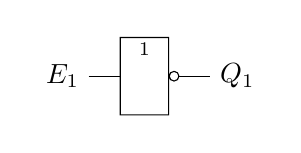
\begin{tikzpicture}[circuit logic IEC]
\matrix[column sep=4mm]
{
\node (i0) {$E_1$}; & \node [not gate] (a) {}; & \node (o) {$Q_1$};\\
};
\draw (i0.east) -- ++(right:3mm) |- (a.input);
\draw (a.output) -- ++(right:3mm) |- (o.west);
\end{tikzpicture} 
&
%% AND
\begin{tikzpicture}[circuit logic IEC]
\matrix[column sep=4mm]
{
\node (i0) {$E_1$}; & 							& \\
				    & \node [and gate] (a) {}; & \node (o) {$Q_1$};\\
\node (i1) {$E_2$}; &							& \\
};
\draw (i0.east) -- ++(right:3mm) |- (a.input 1);
\draw (i1.east) -- ++(right:3mm) |- (a.input 2);
\draw (a.output) -- ++(right:3mm) |- (o.west);
\end{tikzpicture} 
& 
%%OR 
\begin{tikzpicture}[circuit logic IEC]
\matrix[column sep=4mm]
{
\node (i0) {$E_1$}; & 							& \\
				    & \node [or gate] (a) {}; & \node (o) {$Q_1$};\\
\node (i1) {$E_2$}; &							& \\
};
\draw (i0.east) -- ++(right:3mm) |- (a.input 1);
\draw (i1.east) -- ++(right:3mm) |- (a.input 2);
\draw (a.output) -- ++(right:3mm) |- (o.west);
\end{tikzpicture}
& 
%%NAND 
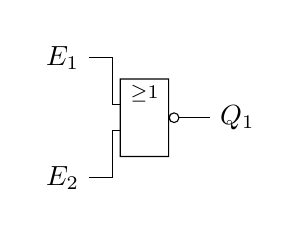
\begin{tikzpicture}[circuit logic IEC]
\matrix[column sep=4mm]
{
\node (i0) {$E_1$}; & 							& \\
				    & \node [nor gate] (a) {}; & \node (o) {$Q_1$};\\
\node (i1) {$E_2$}; &							& \\
};
\draw (i0.east) -- ++(right:3mm) |- (a.input 1);
\draw (i1.east) -- ++(right:3mm) |- (a.input 2);
\draw (a.output) -- ++(right:3mm) |- (o.west);
\end{tikzpicture} \\ \hline 
Wahrheitstabelle   &
%% Negation 
\begin{tabular}{c | c}
$E_1$ & $Q$ \\ \hline
0 & 1 \\ \hline
1 & 0 \\ 
\end{tabular}
& 
%%AND 
\begin{tabular}{c | c | c}
$E_1$ & $E_2$ & $Q$ \\ \hline
0 & 0 & 0 \\ \hline
1 & 0 & 0 \\ \hline
0 & 1 & 0 \\ \hline
1 & 1 & 1 \\
\end{tabular}
& 
%%OR 
\begin{tabular}{c | c | c}
$E_1$ & $E_2$ & $Q$ \\ \hline
0 & 0 & 0 \\ \hline
1 & 0 & 1 \\ \hline
0 & 1 & 1 \\ \hline
1 & 1 & 1 \\
\end{tabular}
& 
%%NAND
\begin{tabular}{c | c | c}
$E_1$ & $E_2$ & $Q$ \\ \hline
0 & 0 & 1 \\ \hline
1 & 0 & 1 \\ \hline
0 & 1 & 1 \\ \hline
1 & 1 & 0 \\
\end{tabular}
\\ \hline
\multirow{2}{*}{Funktionsgleichung} & $\overline{E_1}=Q$ & $E_1 \land E_2 = Q_1$ & $E_1 \lor E_2 = Q_1$ & $\overline{E_1 \land E_2} = Q_1$ \\ 
&&& $\overline{E_1} \lor \overline{E_2} = Q_1$ \\ \hline
Schalteräquivalent & 
%%Negation 
\begin{tikzpicture}[circuit ee IEC]
{
\draw (0,0)node[anchor=east] {$1$} to [break contact={info=$E_1$}] (2,0) node[anchor=west] {$Q_1$};
}
\end{tikzpicture} 
& 
%%AND 
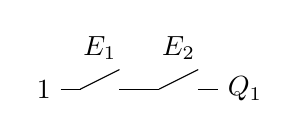
\begin{tikzpicture}[circuit ee IEC]
{
\draw (0,0)node[anchor=east] {$1$} to [make contact={info=$E_1$}] (1,0);
\draw (1,0) to [make contact={info=$E_2$}] (2,0) node[anchor=west] {$Q_1$};
}
\end{tikzpicture}
& 
%%OR 
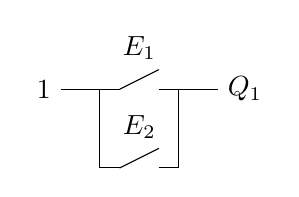
\begin{tikzpicture}[circuit ee IEC]
{
\draw (0,0) node[anchor=east] {$1$} -- (0.5,0);
\draw (0.5,0) -- (0.5,-1);
\draw (1.5,0) -- (1.5,-1);
\draw (0.5,0) to [make contact={info=$E_1$}] (1.5,0);
\draw (0.5,-1) to [make contact={info=$E_2$}] (1.5,-1);
\draw (1.5,0) -- (2,0) node[anchor=west] {$Q_1$};
}
\end{tikzpicture}
& 
%%NAND
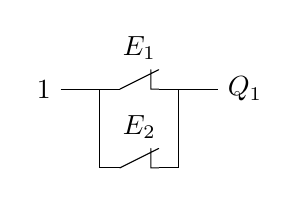
\begin{tikzpicture}[circuit ee IEC]
{
\draw (0,0) node[anchor=east] {$1$} -- (0.5,0);
\draw (0.5,0) -- (0.5,-1);
\draw (1.5,0) -- (1.5,-1);
\draw (0.5,0) to [break contact={info=$E_1$}] (1.5,0);
\draw (0.5,-1) to [break contact={info=$E_2$}] (1.5,-1);
\draw (1.5,0) -- (2,0) node[anchor=west] {$Q_1$};
}
\end{tikzpicture}
\\ \hline
 
\end{tabular}

\newpage

\begin{tabular}{r | l | l | l }
Typ                & NOR & XOR & XNOR \\ \hline
Symbol             &  
%%NOR 
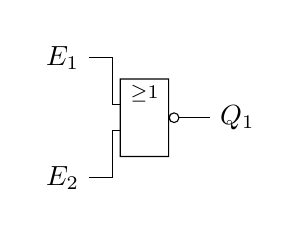
\begin{tikzpicture}[circuit logic IEC]
\matrix[column sep=4mm]
{
\node (i0) {$E_1$}; & 							& \\
				    & \node [nor gate] (a) {}; & \node (o) {$Q_1$};\\
\node (i1) {$E_2$}; &							& \\
};
\draw (i0.east) -- ++(right:3mm) |- (a.input 1);
\draw (i1.east) -- ++(right:3mm) |- (a.input 2);
\draw (a.output) -- ++(right:3mm) |- (o.west);
\end{tikzpicture}
& 
%%EXOR 
\begin{tikzpicture}[circuit logic IEC]
\matrix[column sep=4mm]
{
\node (i0) {$E_1$}; & 							& \\
				    & \node [xor gate] (a) {}; & \node (o) {$Q_1$};\\
\node (i1) {$E_2$}; &							& \\
};
\draw (i0.east) -- ++(right:3mm) |- (a.input 1);
\draw (i1.east) -- ++(right:3mm) |- (a.input 2);
\draw (a.output) -- ++(right:3mm) |- (o.west);
\end{tikzpicture}
& 
%%EXNOR 
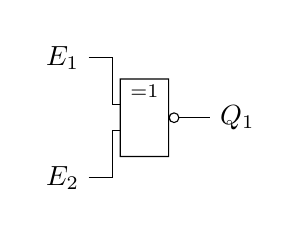
\begin{tikzpicture}[circuit logic IEC]
\matrix[column sep=4mm]
{
\node (i0) {$E_1$}; & 							& \\
				    & \node [xnor gate] (a) {}; & \node (o) {$Q_1$};\\
\node (i1) {$E_2$}; &							& \\
};
\draw (i0.east) -- ++(right:3mm) |- (a.input 1);
\draw (i1.east) -- ++(right:3mm) |- (a.input 2);
\draw (a.output) -- ++(right:3mm) |- (o.west);
\end{tikzpicture}
\\ \hline
Wahrheitstabelle   & 
%%NOR 
\begin{tabular}{c | c | c}
$E_1$ & $E_2$ & $Q$ \\ \hline
0 & 0 & 1 \\ \hline
1 & 0 & 0 \\ \hline
0 & 1 & 0 \\ \hline
1 & 1 & 0 \\
\end{tabular}
& 
%%XOR 
\begin{tabular}{c | c | c}
$E_1$ & $E_2$ & $Q$ \\ \hline
0 & 0 & 0 \\ \hline
1 & 0 & 1 \\ \hline
0 & 1 & 1 \\ \hline
1 & 1 & 0 \\
\end{tabular}
& 
%%XNOR 
\begin{tabular}{c | c | c}
$E_1$ & $E_2$ & $Q$ \\ \hline
0 & 0 & 1 \\ \hline
1 & 0 & 0 \\ \hline
0 & 1 & 0 \\ \hline
1 & 1 & 1 \\
\end{tabular}\\ \hline
Funktionsgleichung & $\overline{E_1} \land \overline{E_2} = Q_1$ & $(E_1 \land \overline{E_2}) \lor (\overline{E_1} \land E_2) = Q_1 $ & $(\overline{E_1} \land \overline{E_2}) \lor (E_1 \land E_2) = Q $ \\ 
&$\overline{E_1 \lor E_2} = Q_1$&& \\ \hline
Schalteräquivalent & 
%%NOR 
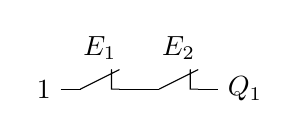
\begin{tikzpicture}[circuit ee IEC]
{
\draw (0,0)node[anchor=east] {$1$} to [break contact={info=$E_1$}] (1,0);
\draw (1,0) to [break contact={info=$E_2$}] (2,0) node[anchor=west] {$Q_1$};
}
\end{tikzpicture}
& 
%%XOR 
\begin{tikzpicture}[circuit ee IEC]
{
%\draw (0,0.75) -- (0.1,0.75);
\draw (0,0)node[anchor=east] {$1$} -- (0.5,0);
\draw (0.5,0) -- (1,-0.5) node [anchor=east] {$E_1$};
\draw (1,-0.5) --  (2,-0.5);
\draw (1,0.5) --  (2,0.5);
\draw (2,0.5)node [anchor=west] {$E_2$} -- (2.5,0);
\draw (2.5,0) -- (3,0) node[anchor=west] {$Q_1$};
}
\end{tikzpicture}
& 
%%XNOR 
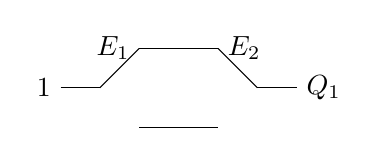
\begin{tikzpicture}[circuit ee IEC]
{
%\draw (0,0.75) -- (0.1,0.75);
\draw (0,0)node[anchor=east] {$1$} -- (0.5,0);
\draw (0.5,0) -- (1,0.5) node [anchor=east] {$E_1$};
\draw (1,-0.5) --  (2,-0.5);
\draw (1,0.5) --  (2,0.5);
\draw (2,0.5)node [anchor=west] {$E_2$} -- (2.5,0);
\draw (2.5,0) -- (3,0) node[anchor=west] {$Q_1$};
}
\end{tikzpicture}
\\ \hline
 
\end{tabular}


\end{landscape}

\subsection{Beispielaufbau XOR}
Um die Schaltfunktion der einzelnen Bausteine überprüfen und die Wahrheitstabellen ausfüllen zu können lassen sich eine vielzahl einfacher Schaltungen aufbauen.
Die Schalteräquivalente stellen diese Schaltungen dar. Etwas spannender ist es das Exklusiv Oder aus einzelnen Invertieren, AND-Gattern und einem OR-Gatter aufzubauen.
\begin{center}
\begin{tikzpicture}[circuit logic IEC]
\matrix[column sep=7mm]
{
\node (i0) {};	& 							& 							& &\\
				& 							& 							& &\\
\node (i1) {};	& \node [not gate](n1){};	& \node [and gate] (a1) {}; & &\\
				& 							&							& \node [or gate] (b) {}; & \node (o) {Q}\\
\node (i2) {};	& \node [not gate](n2){}; 	& \node [and gate] (a2) {};	& &\\
				& 							&							& &\\
\node (i3) {};	& 							&							& &\\
};
\draw (i0.east) -- ++(right:17mm) |- (a1.input 1);
\draw (i1.east) -- ++(right:3mm) |- (n1.input);
\draw (n1.output) -- ++(right:3mm) |- (a1.input2);

\draw (i2.east) -- ++(right:3mm) |- (n2.input);
\draw (n2.output) -- ++(right:3mm) |- (a2.input 1);
\draw (i3.east) -- ++(right:17mm) |- (a2.input 2);

\draw (a1.output) -- ++(right:3mm) |- (b.input 1);
\draw (a2.output) -- ++(right:3mm) |- (b.input 2);

\draw (b.output) -- ++(right:3mm) |- (o.east);

\end{tikzpicture}
\end{center}

\section{Bausteine mit mehreren Eingängen}


%%%
%%% end main document
%%%
%%%%%%%%%%%%%%%%%%%%%%%%%%%%%%%%%%%%%%%%%%%%%%%%%%%%%%%%%%%%%%%%%%%%%%%%%%%%%%%%

% \appendix  %% include it, if something (bibliography, index, ...) follows below

%%%%%%%%%%%%%%%%%%%%%%%%%%%%%%%%%%%%%%%%%%%%%%%%%%%%%%%%%%%%%%%%%%%%%%%%%%%%%%%%
%%%
%%% bibliography
%%%
%%% available styles: abbrv, acm, alpha, apalike, ieeetr, plain, siam, unsrt
%%%
% \bibliographystyle{plain}

%%% name of the bibliography file without .bib
%%% e.g.: literatur.bib -> \bibliography{literatur}
% \bibliography{FIXXME}

\end{document}
%%% }}}
%%% END OF FILE
%%%%%%%%%%%%%%%%%%%%%%%%%%%%%%%%%%%%%%%%%%%%%%%%%%%%%%%%%%%%%%%%%%%%%%%%%%%%%%%%
%%% Notice!
%%% This file uses the outline-mode of emacs and the foldmethod of Vim.
%%% Press 'zi' to unfold the file in Vim.
%%% See ':help folding' for more information.
%%%%%%%%%%%%%%%%%%%%%%%%%%%%%%%%%%%%%%%%%%%%%%%%%%%%%%%%%%%%%%%%%%%%%%%%%%%%%%%%
%% Local Variables:
%% mode: outline-minor
%% OPToutline-regexp: "%% .*"
%% OPTeval: (hide-body)
%% emerge-set-combine-versions-template: "%a\n%b\n"
%% End:
%% vim:foldmethod=marker
